\documentclass{beamer}
\usetheme[deutsch]{KIT}

\usepackage[utf8]{inputenc}
\usepackage[T1]{fontenc}
\usepackage{babel}
\usepackage{tikz,calc,ifthen}
\usepackage{mathtools}
\usepackage[normalem]{ulem}
\usepackage{graphicx}
\usepackage{xspace}
\usepackage{minted}
\usepackage{realboxes}

\usetikzlibrary{positioning,calc,arrows,shapes}
\tikzset{
  every node/.style={transform shape},
  auto,
  block/.style={align=center,rectangle,draw,minimum height=20pt,minimum width=30pt},
  >=triangle 60,
  alt/.code args={<#1>#2#3}{%
      \alt<#1>{\pgfkeysalso{#2}}{\pgfkeysalso{#3}}
  },
  beameralert/.style={alt=<#1>{color=green!80!black}{}},
  mythick/.style={line width=1.4pt}
}

\newcommand*{\maxwidthofm}[2]{\maxof{\widthof{$#1$}}{\widthof{$#2$}}}
\newcommand<>*{\robustaltm}[2]{
  \alt#3
  {\mathmakebox[\maxwidthofm{#1}{#2}]{#1}\vphantom{#1#2}}
    {\mathmakebox[\maxwidthofm{#1}{#2}]{#2}\vphantom{#1#2}}
}

\newcommand<>*{\nodealert}[1]{\only#2{\draw[overlay,mythick,color=green!80!black] (#1.north west) rectangle (#1.south east)}}

%Stuff

\newcommand{\cmark}{\ding{51}}%
\newcommand{\xmark}{\ding{55}}%

% Benchmarks

\newcommand*{\varfull}{\textbf{(1)}\xspace}
\newcommand*{\varedges}{\textbf{(2)}\xspace}
\newcommand{\progname}[1]{\texttt{#1}}
\newcommand{\totalname}[1]{#1}
\newcommand{\andmore}[1]{\emph{... and #1 more}}

%%% Typographic defs

% From https://stackoverflow.com/a/39363004/388010
% Add a period to the end of an abbreviation unless there's one
% already, then \xspace.
\makeatletter
\DeclareRobustCommand\onedot{\futurelet\@let@token\@onedot}
\def\@onedot{\ifx\@let@token.\else.\null\fi\xspace}

\def\eg{e.g\onedot} \def\Eg{E.g\onedot}
\def\ie{i.e\onedot} \def\Ie{I.e\onedot}
\def\cf{c.f\onedot} \def\Cf{C.f\onedot}
\def\etc{etc\onedot} \def\vs{vs\onedot}
\def\wrt{w.r.t\onedot} \def\dof{d.o.f\onedot}
\def\etal{et al\onedot}
\makeatother

\newcommand{\newdef}[1]{\emph{#1}}

\newcommand{\anal}[1]{\textsc{#1}\xspace}
\newcommand*{\MayAlias}{\anal{MayAlias}}
\newcommand*{\MustAlias}{\anal{MustAlias}}
\newcommand*{\MinCard}{\anal{MinCard}}
\newcommand*{\MaxCard}{\anal{MaxCard}}

%%% Minted for syntax highlighting

\newmintinline[hs]{haskell}{}
\newminted[haskell]{haskell}{linenos,mathescape,texcomments,autogobble}

% Syntax
\newcommand{\keyword}[1]{\text{\textsf{\textbf{#1}}}}
\newcommand{\sMkPair}{\text{\textsf{(,)}}}
\newcommand{\sApp}[2]{#1\,#2}
\newcommand{\sLam}[2]{\lambda{}#1.\,#2}
\newcommand{\sLet}[2]{\keyword{let}~#1~\keyword{in}~#2}
\newcommand{\sLetRec}[2]{\keyword{letrec}~#1~\keyword{in}~#2}
\newcommand{\sPair}[2]{(#1,#2)}
\newcommand{\sCase}[4]{\keyword{case}~#1~\keyword{of}~\sPair{#2}{#3}\rightarrow#4}
\newcommand{\sITE}[3]{\keyword{if}~#1~\keyword{then}~{#2}~\keyword{else}~{#3}}

\newcommand{\bind}{x_1=e_1}
\newcommand{\binds}{\overline{x_i=e_i}}

% Co-call Graphs
\newcommand{\edge}[2]{#1\text{---}#2}
\newcommand{\neighbors}[2]{N_{#1} ({#2})}

% Semantic sets
\newcommand{\sVar}{\text{\textsf{Var}}}
\newcommand{\sTrue}{\text{\textsf{True}}}
\newcommand{\sFalse}{\text{\textsf{False}}}
\newcommand{\sExp}{\text{\textsf{Exp}}}
\newcommand{\sVal}{\text{\textsf{Val}}}
\newcommand{\sGraph}{\text{\textsf{Graph}}}
\newcommand{\sUse}{\text{\textsf{Use}}}
\newcommand{\sUsage}{\text{\textsf{Usage}}}
\newcommand{\sMulti}{\text{\textsf{Multi}}}
\newcommand{\sSig}{\text{\textsf{Sig}}}
\newcommand{\sUseEnv}{\text{\textsf{UseEnv}}}
\newcommand{\sUType}{\text{\textsf{UType}}}
\newcommand{\sUTrans}{\text{\textsf{UTrans}}}
\newcommand{\sTransEnv}{\text{\textsf{TransEnv}}}

% Lattice

\newcommand{\llub}{\sqcup}
\newcommand{\lbiglub}{\bigsqcup}
\newcommand{\lleq}{\sqsubseteq}
\newcommand{\lless}{\sqsubset}
\newcommand{\lPair}[2]{\left\langle{}#1,#2\right\rangle{}}
\newcommand{\lTriple}[3]{\left\langle{}#1,#2,#3\right\rangle{}}
\newcommand{\both}{\,\&\,}
\newcommand{\mto}{\to_{+}}

% Transfer function
\newcommand{\transfer}[2]{\mathcal{T}\llbracket#1\rrbracket_{#2}}
\newcommand*{\letupsc}{\textsc{LetUp}\xspace}
\newcommand*{\letdnsc}{\textsc{LetDn}\xspace}
\newcommand{\fix}{\keyword{fix}\xspace}
\newcommand{\up}{\sfop{up}}
\newcommand{\down}{\sfop{down}}

% Auxiliary

% https://tex.stackexchange.com/a/268475/52414
\newlength\stextwidth
\newcommand\makesamewidth[3][c]{%
  \settowidth{\stextwidth}{#2}%
  \makebox[\stextwidth][#1]{#3}%
}
\newlength\smathtextwidth
\newcommand\mathmakesamewidth[3][c]{%
  \settowidth{\smathtextwidth}{$#2$}%
  \mathmakebox[\smathtextwidth][#1]{#3}%
}
\newcommand\mathwithin[2]{%
  \mathmakesamewidth[c]{#1}{#2}
}

\definecolor{mygreen}{HTML}{6aa84f}
\newcommand{\sfop}[1]{\mathsf{#1}}
\newcommand{\uscore}[1][\mathunderscore]{\mathwithin{#1}{\mathunderscore}}
\newcommand{\expand}{\sfop{expand}}
\newcommand{\dom}[1]{\sfop{dom}\,#1}
\newcommand{\zap}{\sfop{zap}}
\newcommand{\letup}[2]{#1\!\uparrow_{#2}}
\newcommand{\letdown}[2]{#1\!\downarrow_{#2}}
\newcommand{\liftstar}[1]{[#1]^*}
\newcommand{\liftqm}[1]{[#1]^\sfop{?}}
\newcommand{\cmblet}[2]{#1\ltimes#2}

% Map Notation
\newcommand{\pfun}{\rightharpoonup}
\newcommand{\emptymap}{[]}
\newcommand{\id}[1]{#1}
\newcommand{\maplit}[3][\id]{\left[#1{#2\mapsto#3}\right]}
\newcommand{\restrict}[2]{#1\restriction_{#2}}


\title{Call Arity vs. Demand Analysis}
\author{Sebastian Graf}
\subtitle{\insertauthor}
\institute[IPD]{Lehrstuhl Programmierparadigmen, IPD Snelting}
\date{9.8.2017}
\KITtitleimage{cover.png}

\begin{document}

\begin{frame}
  \maketitle
\end{frame}

\begin{frame}{Motivation}
  \begin{itemize}
    \item Glasgow Haskell Compiler (GHC): >100k lines of code
    \item Typical challenges of big software projects
    \item Two analyses with overlapping concerns
      \begin{itemize}
        \item Demand Analyser
        \item Call Arity
      \end{itemize}
    \item Extract overlaps into combined analysis
      \begin{itemize}
        \item Both prior analyses profit from increased precision
        \item Principle of DRY
      \end{itemize}
  \end{itemize}
\end{frame}

\begin{frame}[fragile]{Cardinality Analysis}
  \begin{itemize}
    \item 
      Provides lower and upper bounds on \emph{evaluation cardinality}
      \begin{itemize} \item \MinCard and \MaxCard analyses \end{itemize}
    \item Notation: $[n,m]$, where $n,m \in \{0,1,\omega\}, n \leq m$
  \end{itemize}
  \begin{center}
    \begin{minipage}{0.5\textwidth}
      \begin{haskell}
        main = do
          let a = ... -- $[1,\omega]$
              b = ... -- $[1,1]$
              c = ... -- $[0,\omega]$
              d = ... -- $[0,1]$
              e = ... -- $[0,0]$
          print (a + if b then a * d else c * c)
      \end{haskell}
    \end{minipage}
  \end{center}
\end{frame}

\begin{frame}[fragile]{Call-by-value}
  \begin{itemize}
    \item 
      Avoids operational complexity of laziness, enables unboxing
      \begin{itemize} \item Exploits \emph{strictness} \end{itemize}
      \begin{itemize} \item `Evaluated at \emph{least} once' (\MinCard) \end{itemize}
  \end{itemize}
  \begin{center}
    \begin{minipage}{0.5\textwidth}
      \begin{haskell}
        main = do
          let !a    = ...                 -- $[\mathbf{1},\omega]$
              !b    = ...                 -- $[\mathbf{1},1]$
               c    = ...                 -- $[0,\omega]$
               d    = ...                 -- $[0,1]$
               e    = ...                 -- $[0,0]$
          print (a + if b then a * d else c * c)
      \end{haskell}
    \end{minipage}
  \end{center}
\end{frame}

\begin{frame}[fragile]{Call-by-name}
  \begin{itemize}
    \item 
      Omits updates of \emph{single-entry} thunks, mimicing regular function calls
      \begin{itemize} \item Exploits lack of \emph{sharing} \end{itemize}
      \begin{itemize} \item `Evaluated at \emph{most} once' (\MaxCard) \end{itemize}
  \end{itemize}
  \begin{center}
    \begin{minipage}{0.5\textwidth}
      \begin{haskell}
        main = do
          let  a    = ...                 -- $[1,\omega]$
               b () = ...                 -- $[1,\mathbf{1}]$
               c    = ...                 -- $[0,\omega]$
               d () = ...                 -- $[0,\mathbf{1}]$
               e () = ...                 -- $[0,\mathbf{0}]$
          print (a + if b () then a * d () else c * c)
      \end{haskell}
    \end{minipage}
  \end{center}
\end{frame}

\begin{frame}[fragile]{Dead code}
  \begin{itemize}
    \item Can replace dead bindings with small traps
    \begin{itemize} \item Exploits \emph{absence} \end{itemize}
    \begin{itemize} \item `Never evaluated' (\MaxCard) \end{itemize}
  \end{itemize}
  \begin{center}
    \begin{minipage}{0.5\textwidth}
      \begin{haskell}
        main = do
          let  a    = ...                 -- $[1,\omega]$
               b    = ...                 -- $[1,1]$
               c    = ...                 -- $[0,\omega]$
               d    = ...                 -- $[0,1]$
               e    = error "e is absent" -- $[0,\mathbf{0}]$
          print (a + if b then a * d else c * c)
      \end{haskell}
    \end{minipage}
  \end{center}
\end{frame}

\begin{frame}[fragile]{Usage Analysis}
  \begin{itemize}
    \item \MaxCard analysis, \eg computes $m$ in binding annotations $[n,m]$
    \item 
      Related: \emph{one-shot} lambdas
  \end{itemize}
  \begin{center}
    \begin{minipage}{0.5\textwidth}
      \begin{haskell*}{escapeinside=||}
        main = do        
          let c = ...
              f = \|$\mathtt{x}^\omega$| |$\mathtt{y}^1$| -> c*x + y
              g = \|$\mathtt{z}^1$| -> 
                    let d = ... 
                    in \|$\mathtt{w}^1$| -> c*d + z*w
          print (f 1 2 + f 4 5 * g 3 42)
      \end{haskell*}
    \end{minipage}
  \end{center}
\end{frame}

% Proably backup, also useful to explain inlining
\begin{frame}[fragile]{Floating}
  \begin{itemize}
    \item Floating bindings in and out of expressions
    \item Floating into a lambda possibly duplicates work!
    \item Not so with one-shot lambdas
  \end{itemize}
  \begin{center}
    \begin{minipage}{0.5\textwidth}
      \begin{overprint}
        \onslide<1>
        \begin{haskell*}{escapeinside=||}
          main = do        
            let c = ...
                f = \|$\mathtt{x}^\omega$| |$\mathtt{y}^1$| -> c*x + y
                g = \|$\mathtt{z}^1$| -> 
                      let d = ... 
                      in \|$\mathtt{w}^1$| -> c*d + z*w
            print (f 1 2 + f 4 5 * g 3 42)
        \end{haskell*}
        \onslide<2>
        \begin{haskell*}{escapeinside=||}
          main = do        
            let |\color{red}\texttt{c}| = ...
                f = \|$\mathtt{x}^{\color{red} \omega}$| |$\mathtt{y}^1$| -> |\color{red}\texttt{c}|*x + y
                g = \|$\mathtt{z}^1$| -> 
                      let d = ... 
                      in \|$\mathtt{w}^1$| -> |\color{red}\texttt{c}|*d + z*w
            print (f 1 2 + f 4 5 * g 3 42)
        \end{haskell*}
        \onslide<3>
        \begin{haskell*}{escapeinside=||}
          main = do        
            let c = ...
                f = \|$\mathtt{x}^\omega$| |$\mathtt{y}^1$| -> c*x + y
                g = \|$\mathtt{z}^1$| -> 
                      let |\color{red}\texttt{d}| = ... 
                      in \|$\mathtt{w}^1$| -> c*|\color{red}\texttt{d}| + z*w
            print (f 1 2 + f 4 5 * g 3 42)
        \end{haskell*}
        \onslide<4>
        \begin{haskell*}{escapeinside=||}
          main = do        
            let c = ...
                f = \|$\mathtt{x}^\omega$| |$\mathtt{y}^1$| -> c*x + y
                g = \|$\mathtt{z}^1$| |$\mathtt{w}^1$| -> 
                      let |\color{red}\texttt{d}| = ... 
                      in c*|\color{red}\texttt{d}| + z*w
            print (f 1 2 + f 4 5 * g 3 42)
        \end{haskell*}
      \end{overprint}
    \end{minipage}
  \end{center}
\end{frame}

\begin{frame}[fragile]{$\eta$-Expansion}
  \begin{itemize}
    \item Floats lambdas out, possibly duplicating work
    \item Not so with one-shot lambdas
  \end{itemize}
  \begin{center}
    \begin{minipage}{0.5\textwidth}
      \begin{overprint}
        \onslide<1>
        \begin{haskell*}{escapeinside=||}
          main = do        
            let g = \|$\mathtt{z}^1$| -> 
                      let d = ... 
                      in \|$\mathtt{w}^{\color{red} 1}$| -> d + z*w
            print (g 3 42)
        \end{haskell*}
        \onslide<2>
        \begin{haskell*}{escapeinside=||}
          main = do        
            let g = \|$\mathtt{z}^1$| \|\color{red}$\mathtt{w}^1$| -> 
                      let d = ... 
                      in d + z*w
            print (g 3 42)
        \end{haskell*}
      \end{overprint}
    \end{minipage}
  \end{center}
\end{frame}

\begin{frame}[fragile]{Demand Analyser}
  \begin{overprint}
    \onslide<1>
    \begin{itemize}
      \item A cardinality analysis
      \item Usage analysis identifies
        \begin{itemize}
          \item Single-entry thunks
          \item One-shot lambdas
          \item Dead code
        \end{itemize}
      \item Computes how an expression uses its free variables
    \end{itemize}

    \onslide<2>
    \begin{itemize}
      \item Call Uses
        \begin{itemize}
          \item Identification of one-shot lambdas needs tracking of \emph{how} a binding was used
          \item Introduces \newdef{call uses} $C^n(u)$
          \item \hs{f 1 2} exposes \hs{f} to usage $1*C^1(C^1(U))$
          \item \hs{f 1 2 + f 4 5} exposes \hs{f} to usage $\omega*C^\omega(C^1(U))$
        \end{itemize}
    \end{itemize}
    \begin{center}
      \begin{minipage}{0.5\textwidth}
        \begin{haskell*}{escapeinside=||}
          let f |$\mathtt{x}^\omega$| |$\mathtt{y}^1$| = ...
          in f 1 2 + f 4 5
        \end{haskell*}
      \end{minipage}
    \end{center}

    \onslide<3>
    \begin{itemize}
      \item Usage Signatures
        \begin{itemize}
          \item Interprocedural data-flow
          \item \hs{const} has \newdef{usage signature} $1*U \to A \to \bullet$
          \item \hs{y} is used once, $1*U$
          \item \hs{fac 1000} is dead code ($A$ for absent, \eg never used)
          \item Usage signature + free variable usage = \newdef{usage type}
          \item Looks at the definition of \hs{const} before the \hs{let} body!
            \begin{itemize} 
              \item \textsc{LetDn} rule: Unleashes usage types of \hs{const} at call sites
            \end{itemize}
        \end{itemize}
    \end{itemize}
    \begin{center}
      \begin{minipage}{0.5\textwidth}
        \begin{haskell*}{escapeinside=||}
          let const a b = a
          in const y (fac 1000)
        \end{haskell*}
      \end{minipage}
    \end{center}

    \onslide<4>
    \begin{itemize}
      \item Thunks
        \begin{itemize}
          \item \hs{x} is only used once, its evaluation in \hs{y}'s right-hand side is shared!
          \item 
            Two use sites 
            \begin{itemize} 
              \item \textsc{LetDn}-style leads to usage of $\omega*U$ on \hs{x}! 
            \end{itemize}
          \item Solution: \textsc{LetUp} for thunks
            \begin{itemize} 
              \item Record usage $\omega*U$ of \hs{y} in the body of the \hs{let}
              \item Analyse \hs{y}'s bound expression in use $U$, unleash its usage type
            \end{itemize}
        \end{itemize}
    \end{itemize}
    \begin{center}
      \begin{minipage}{0.5\textwidth}
        \begin{haskell*}{escapeinside=||}
          let y = 2*x
          in y + y
        \end{haskell*}
      \end{minipage}
    \end{center}
 \end{overprint}
\end{frame}

\begin{frame}[fragile]{Call Arity}
  \begin{overprint}
    \onslide<1>
    \begin{itemize}
      \item $\eta$-expansion based on usage information
      \item \hs{f} is always called with two arguments
      \item<2> \hs{f}'s bound expression can be $\eta$-expanded!
    \end{itemize}
    \begin{center}
      \begin{minipage}{0.5\textwidth}
        \begin{haskell}
          let f x = 
                if expensive
                then id
                else (*x)
          in f 1 2 + f 4 5
        \end{haskell}
      \end{minipage}
    \end{center}

    \onslide<2>
    \begin{itemize}
      \item $\eta$-expansion based on usage information
      \item \hs{f} is always called with two arguments
      \item<2> \hs{f}'s bound expression can be $\eta$-expanded!
    \end{itemize}
    \begin{center}
      \begin{minipage}{0.5\textwidth}
        \begin{haskell}
          let f x y = 
                if expensive
                then y
                else y*x
          in f 1 2 + f 4 5
        \end{haskell}
      \end{minipage}
    \end{center}

    \onslide<3>
    \begin{itemize}
      \item Can we $\eta$-expand \hs{f} here?
      \item \hs{f} is always called with two arguments
      \item<4> ... but \hs{f} is also a thunk! 
      \item<4> $\eta$-expansion would duplicate the \hs{expensive} check!
    \end{itemize}
    \begin{center}
      \begin{minipage}{0.5\textwidth}
        \begin{haskell}
          let f = 
                if expensive
                then \x y -> y
                else \x y -> y*x
          in f 1 2 + f 4 5
        \end{haskell}
      \end{minipage}
    \end{center}

    \onslide<4>
    \begin{itemize}
      \item Can we $\eta$-expand \hs{f} here?
      \item \hs{f} is always called with two arguments
      \item<4> ... but \hs{f} is also a thunk
      \item<4> $\eta$-expansion would duplicate the \hs{expensive} check!
    \end{itemize}
    \begin{center}
      \begin{minipage}{0.5\textwidth}
        \begin{haskell}
          let f = 
                if expensive
                then \x y -> y
                else \x y -> y*x
          in f 1 2 + f 4 5
        \end{haskell}
      \end{minipage}
    \end{center}

    \onslide<5>
    \begin{itemize}
      \item Can we $\eta$-expand \hs{f} here?
      \item \hs{f} is a thunk, called with two arguments
      \item<6> Since \hs{f} is \emph{called} only \emph{once}, $\eta$-expansion is safe
    \end{itemize}
    \begin{center}
      \begin{minipage}{0.5\textwidth}
        \begin{haskell}
          let f = 
                if expensive
                then \x y -> y
                else \x y -> y*x
          in if b then f 1 2 else f 4 5
        \end{haskell}
      \end{minipage}
    \end{center}

    \onslide<6>
    \begin{itemize}
      \item Can we $\eta$-expand \hs{f} here?
      \item \hs{f} is a thunk, called with two arguments
      \item<6> Since \hs{f} is only \emph{called once}, $\eta$-expansion is safe
      % Also demnostrates why we can't generally just inline \hs{f}
    \end{itemize}
    \begin{center}
      \begin{minipage}{0.5\textwidth}
        \begin{haskell}
          let f x y = 
                if expensive
                then y
                else y*x
          in if b then f 1 2 else f 4 5
        \end{haskell}
      \end{minipage}
    \end{center}

    \onslide<7>
    \begin{itemize}
      \item Called-once information is tracked by a usage analysis
      \item Analyses \hs{let} body before bound expression, bottom-up, like \textsc{LetUp}
      \item Ordinary \textsc{LetUp}-style usage analysis too imprecise
        \begin{itemize}
          \item Forgets that \hs{x} and \hs{y} were evaluated on different code paths
          \item Analysis reports \hs{x} to be used multiple times
        \end{itemize}
    \end{itemize}
    \begin{center}
      \begin{minipage}{0.5\textwidth}
        \begin{haskell}
          let x = ...  
          in let y = 2*x
             in if b
                then x
                else y
        \end{haskell}
      \end{minipage}
    \end{center}

    \onslide<8>
    \begin{itemize}
      \item \emph{Co-call graphs} track control flow information
        \begin{itemize}
          \item Edges connect variables possible evaluated on the same code path
          \item Absence of an edge proves mutual exclusive calls
          \item Usage information in self-edges
        \end{itemize}
      \item Lack of edge between \hs{x} and \hs{y} avoids self-edge on \hs{x}
    \end{itemize}
    \begin{columns}
      \begin{column}{0\textwidth}
        \begin{haskell}
          let x = ...  
          in let y = 2*x
             in if b
                then x
                else y
        \end{haskell}
      \end{column}
      \begin{column}[t]{0\textwidth}
        \vspace{0pt}
        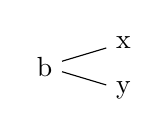
\begin{tikzpicture}
          \node at (0,0) (0) {\hs{b}};
          \node at (1,0.3) (1) {\hs{x}};
          \node at (1,-0.3) (2) {\hs{y}};
          \draw (0) -- (1);
          \draw (0) -- (2);
        \end{tikzpicture}
      \end{column}
    \end{columns}

    \onslide<9>
    \begin{itemize}
      \item \emph{Co-call graphs} track control flow information
        \begin{itemize}
          \item Edges connect variables possible evaluated on the same code path
          \item Absence of an edge proves mutual exclusive calls
          \item Usage information in self-edges
        \end{itemize}
      \item Lack of edge between \hs{x} and \hs{y} avoids self-edge on \hs{x}
    \end{itemize}
    \begin{columns}
      \begin{column}{0\textwidth}
        \begin{haskell}
          let x = ...  
          in let y = 2*x
             in if b
                then x
                else y
        \end{haskell}
      \end{column}
      \begin{column}[t]{0\textwidth}
        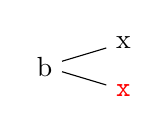
\begin{tikzpicture}
          \node at (0,0) (0) {\hs{b}};
          \node at (1,0.3) (1) {\hs{x}};
          \node at (1,-0.3) (2) {\color{red}\texttt{x}};
          \draw (0) -- (1);
          \draw (0) -- (2);
        \end{tikzpicture}
      \end{column}
    \end{columns}

    \onslide<10>
    \begin{itemize}
      \item \emph{Co-call graphs} track control flow information
        \begin{itemize}
          \item Edges connect variables possible evaluated on the same code path
          \item Absence of an edge proves mutual exclusive calls
          \item Usage information in self-edges
        \end{itemize}
      \item Lack of edge between \hs{x} and \hs{y} avoids self-edge on \hs{x}
    \end{itemize}
    \begin{columns}
      \begin{column}{0\textwidth}
        \begin{haskell}
          let x = ...  
          in let y = 2*x
             in if b
                then x
                else y
        \end{haskell}
      \end{column}
      \begin{column}[t]{0\textwidth}
        \begin{tikzpicture}
          \node at (0,0) (0) {\hs{b}};
          \node at (1,0) (1) {\hs{x}};
          \draw (0) -- (1);
        \end{tikzpicture}
      \end{column}
    \end{columns}
  \end{overprint}
\end{frame}



\begin{frame}{Inhalt}
Idealerweise ein durchgehendes Beispiel benutzen
mit dem man sowohl das Problem, die Lösung, und evtl. Randfälle erklären kann.
\vfill

Der Erfahrung nach braucht man 1-2 Minuten pro Folie.
Für einen 20 Minuten Vortrag sollten es also weniger als 20 Folien sein.
\vfill

Arbeitsaufwand knapp quantifizieren (Lines of Code, Anzahl Theoreme)
\vfill

Was nicht im Vortrag kommt geht unter!
Die Existenz nicht vortrags-fähiger Teile der Arbeit
(wie etwa länglicher Beweise) zumindest erwähnen.
\end{frame}

\begin{frame}{Vorkenntnisse}
Was man bei uns am Lehrstuhl voraussetzen kann:
\vspace{20pt}
\begin{itemize}
  \item libFirm/SSA Form auf einer Folie kurz einführen
  \item C, Java, Haskell, Lambda ist bekannt
  \item X10, ML, Agda, Scala kurz einführen
  \item Andere Programmiersprachen gut motivieren
\end{itemize}
\end{frame}

\begin{frame}{Vortrag}
Alleine Üben! Daheim vor dem Spiegel üben.
Einen Vortrag nur alleine, aber im Stehen und laut sprechend,
vorzutragen ist meist schon lehrreich im Vergleich
zu stillem Folienbasteln.
\vfill

Frei sprechen (oder zumindest die Illusion wahren)
\vfill

Laut und deutlich sprechen (leider häufiges Informatikerproblem)
\vfill

Live vorführen von implementierten, sofern gut geübt, macht Eindruck
\vfill

Zeitrahmen \textbf{nicht überziehen}!
Zwischenfragen gehen natürlich nicht vom Zeitkonto ab
\vfill

Die Folien dem Betreuer zur Durchsicht geben
\end{frame}

\begin{frame}{Bewertung}
\begin{itemize}
  \item Ca.\ 20\% der Gesamtnote kommen durch
    kommunikative soft-skill Aspekte zustande.
  \item Ein schlechter Vortrag kann leicht die Note um 0.7 nach unten ziehen.
\end{itemize}
\end{frame}

\begin{frame}{Links}
\begin{itemize}
  \item \href{http://beza1e1.tuxen.de/articles/technical_presentation.html}{9 Tips how to give a technical presentation}
  \item \href{http://andreas-zeller.blogspot.de/2013/10/summarizing-your-presentation-with.html}{Summarizing your presentation with miniature slides}
  \item \href{https://www.cs.cmu.edu/~kayvonf/misc/cleartalktips.pdf}{Tips for Giving Clear Talks}
\end{itemize}
\end{frame}

\end{document}
